\documentclass[a4paper,12pt]{scrartcl}
\usepackage[utf8x]{inputenc}
\usepackage[T1]{fontenc} % avec T1 comme option  d'encodage c'est ben mieux, surtout pour taper du français.
%\usepackage{lmodern,textcomp} % fortement conseillé pour les pdf. On peut mettre autre chose : kpfonts, fourier,...
\usepackage[french]{babel} %Sans ça les guillemets, amarchpo
\usepackage{amsmath}
\usepackage{multicol}
\usepackage{amssymb}
\usepackage{tkz-tab}
\usepackage{exercice_sheet}

%\trait
%\section*{}
%\exo{}
%\question{}
%\subquestion{}

\date{}


% Title Page
\title{Devoir en classe 1, CG-1, corrigé}

\author{Mathématiques}

\begin{document}

\maketitle

\exo{Résoudre les équations suivantes:}

\question{}
$x^2-x-2=0$

$\Delta = b^2-4ac$.

Ici: $\Delta = (-1)^2-4 \times 1 \times (-2) = 9$.

Donc: $\sqrt{\Delta} = \sqrt{9} = 3$

On a donc $x_1 = \frac{1-3}{2} = -1$

et: $x_2 = \frac{1+3}{2} = 2$.

On a donc $S = \left\lbrace -1 ; 2 \right\rbrace$

\question{}
$x^2+2x+2=0$

Ici, $\Delta = -4 < 0$. $\Delta$ étant négatif, $S = \emptyset$

\exo{Factoriser les expressions suivantes:}

\question{}
$f(x) = x^2 - 4x$

On remarque que $x$ est facteur commun. On peut donc écrire $f(x) = x(x-4)$.

\question{}
$h(x) = x^2-x-2=0$

On remarque qu'il s'agit du même polynôme qu'à la question 1 de l'exercice 1. On en connaît donc les racines, $-1$ et $2$. De plus, $a = 1$. On peut donc le factoriser comme suit: $h(x) = (x+1)\left(x - 2\right)$.

\exo{Statistiques à une variable:}

Nous avons mesuré la taille en centimètres de 11 personnes et réuni les données mesurées dans un tableau:

\begin{center}
\begin{tabular}{|l|l|l|l|l|l|l|l|l|l|l|l|}
\hline
$x_i$ & 164 & 175 & 178 & 181 & 183 & 186 & 189 & 189 & 194 & 197 & 200 \\ \hline
\end{tabular}
\end{center}

Indiquer:

\question{}
L'étendue

$200 - 164 = 36$cm.

\question{}
La médiane $Q_2$

L'effectif étant de 11, on regarde le 6ème terme de la série triée dans l'ordre croissant: 186 cm.

\question{}
Le premier quartile $Q_1$, le troisième quartile $Q_3$

\littlestar{$Q_1$}
$11 \times 0.25 = 2.75$. Les tailles étant triées dans l'ordre croissant, on regarde le 3ème terme: 178 cm.

\littlestar{$Q_3$}
$11 \times 0.75 = 8.25$. Les tailles étant triées dans l'ordre croissant, on regarde le 9ème terme: 194 cm.

\question{}
La moyenne $\overline{x}$

$\overline{x} = \dfrac{164+175+\ldots+200}{11} = 188.1$ cm.

\question{}
La variance $V_x$ et l'écart-type $\sigma_x$. On rappelle que la variance peut se calculer comme suit: $V_x = \overline{x^2} - \overline{x}^2$.

$V_x = \dfrac{164^2+175^2+\ldots+200^2}{11} - \overline{x}^2 = 99.4$

$\sigma_x = \sqrt{V_x} = 9.97$ cm.

\question{}
Quel pourcentage de cette population se situe dans l'intervalle $[\overline{x} - \sigma_x ; \overline{x} + \sigma_x]$?

$\overline{x} - \sigma_x = 178.11$ et $\overline{x} + \sigma_x = 198.07$. Il y a 7 personnes comprises entre ces 2 tailles sur un total de 11. On a donc un pourcentage de $\dfrac{7}{11} \approx 63.6 \%$.

\exo{Statistiques à deux variables}

On veut étudier s'il existe une dépendance entre le nombre de fruits sur un rameau d'un arbre fruitier et la masse de chaque fruit. 

On a relevé sur différents rameaux le nombre de fruits et le poids de chaque fruit. 

Les données relevées sont visibles dans le tableau ci-dessous:

\begin{center}
\begin{tabular}{|l|l|l|l|l|l|l|}
\hline
Nombre de fruits $x_i$       & 1   & 2   & 3   & 4   & 5  & 6  \\ \hline
Poids en grammes $y_i$ & 152 & 147 & 106 & 107 & 77 & 46 \\ \hline
\end{tabular}
\end{center}

\question{}
En prenant 1cm pour une unité en abscisse et 1cm pour 20 grammes en ordonnée, tracer le nuage de points sur votre copie.

\begin{center}
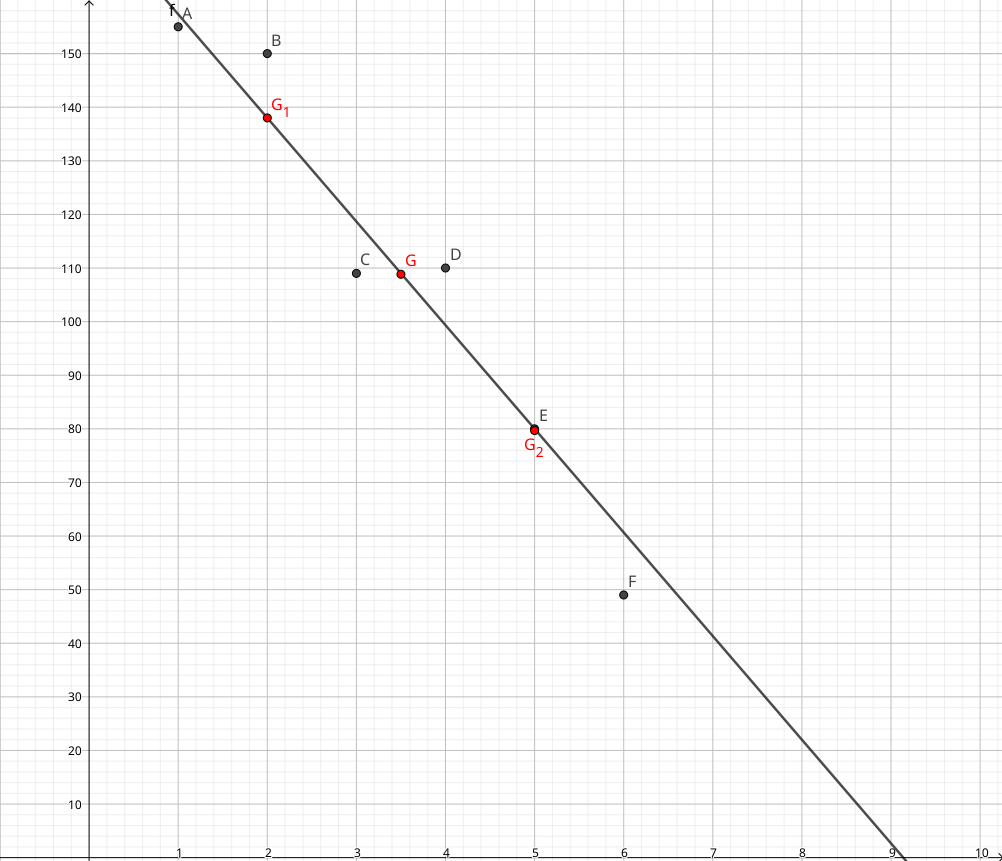
\includegraphics[width=0.7\textwidth]{pics/graphe.pdf}
\end{center}

\question{}
Calculer les coordonnées du point moyen $G$ et le tracer sur le graphe.

On rappelle que les coordonnées de $G$ sont: $G(\overline{x},\overline{y})$.

On calcule donc la moyenne de chaque variable et obtient $G(3.5,105.83)$

\question{}
Méthode de Mayer

\subquestion{}
Calculer les coordonnées du point $G_1$, point moyen des trois premiers points ainsi que celles de $G_2$, point moyen des trois derniers points du nuage. 

Pour $G_1$ on calcule les coordonnées en calculant la moyenne de chaque variable sur les 3 premières colonnes du tableau: $G_1(2;135)$.

Pour $G_2$ on calcule les coordonnées en calculant la moyenne de chaque variable sur les 3 dernières colonnes du tableau: $G_2(5;76.67)$.

\subquestion{}
Tracer $G_1$ et $G_2$ sur le graphe.

\subquestion{}
Indiquer l'équation de la droite $(G_1 G_2)$ et la tracer sur le graphe. 

$(G_1 G_2):y=ax+b$, on cherche $a$ et $b$. Chaque point $G_1$ et $G_2$ va nous donner une équation, on obtient donc un système de 2 équations à 2 inconnues:

$$
\begin{cases} 
2 a + b &= 135 \\
5 a + b &= 76.67
\end{cases}
$$

On se propose de multiplier la 2ème ligne par $-1$ afin d'éliminer $b$ par addition des 2 lignes.

$$
\begin{cases} 
2 a + b &= 135 \\
-5 a - b &= -76.67
\end{cases}
$$

On obtient donc:

$$-3a = 58.33 \Leftrightarrow a = -19.44$$

On utilise la valeur trouvée de $a$ dans (par exemple) la 1re équation: $$2 \times (-19.44) + b = 138 \Leftrightarrow b = 135 + 38.887 \approx 173.9$$

On obtient donc l'équation de $(G_1 G_2):y = -19.44 x + 173.9$. 

\subquestion{}
En utilisant l'équation de cette droite, quelle masse peut-on attendre pour un fruit issu d'un rameau contenant 8 fruits?

On utilise l'équation de $(G_1 G_2)$ en posant $x=8$. On obtient donc $y = -19.44 \times 8 + 176.89 \approx 18$g.

La méthode de Mayer prédit donc qu'un fruit issu d'une branche en contenant 8 pèsera 18 grammes.

\trait

\begin{center}
Fin.
\end{center}

\end{document}
